%% ==========================================================================
%%  Matryoshka-ECG -- REVISED MANUSCRIPT (major revision resubmission)
%%  IEEE Journal of Biomedical and Health Informatics
%%
%%  Build:   latexmk -pdf main.tex        (or: make)
%%
%%  NUMBERS POLICY
%%  --------------
%%  Every quantitative result is a macro defined in generated/numbers.tex,
%%  which is written by code/scripts/aggregate_results.py from the actual
%%  experiment outputs. Until the pipeline is run, undefined macros render as
%%  a visible red [TBD] rather than a plausible-looking number. Do not
%%  hard-code results into this file.
%% ==========================================================================
\documentclass[journal,twoside]{IEEEtran}

\usepackage{cite}
\usepackage{amsmath,amssymb,amsfonts}
\usepackage{algorithm}
\usepackage{algpseudocode}
\usepackage{graphicx}
\usepackage{booktabs}
\usepackage{multirow}
\usepackage{url}
\usepackage{xcolor}
\usepackage[hidelinks]{hyperref}
\usepackage{balance}

\graphicspath{{figures/}}

% --------------------------------------------------------------------------
% Placeholder machinery: any result macro that has not yet been generated
% renders as a conspicuous [TBD] so that no invented number can survive to
% submission.
% --------------------------------------------------------------------------
\newcommand{\TBD}{\textcolor{red}{\textbf{[TBD]}}}
\makeatletter
\newcommand{\R}[1]{\@ifundefined{#1}{\TBD}{\csname #1\endcsname}}
\makeatother
\IfFileExists{generated/numbers.tex}{% AUTO-GENERATED by scripts/aggregate_results.py -- do not edit
\newcommand{\DimLarge}{512}
\newcommand{\DimSmall}{16}
\newcommand{\EffRank}{16.7}
\newcommand{\EquivDiff}{0.0013}
\newcommand{\EquivHi}{0.0019}
\newcommand{\EquivLo}{0.0007}
\newcommand{\EquivMargin}{0.010}
\newcommand{\EquivVerdict}{statistically equivalent}
\newcommand{\GPUName}{NVIDIA L4}
\newcommand{\HierP}{0.224}
\newcommand{\HierRho}{0.399}
\newcommand{\HierVerdict}{not supported}
\newcommand{\IncAUClarge}{0.9263}
\newcommand{\IncAUCsmall}{0.9269}
\newcommand{\IncParams}{4,595,022}
\newcommand{\IncSDlarge}{0.0021}
\newcommand{\IncSDsmall}{0.0018}
\newcommand{\IncSpread}{0.0005}
\newcommand{\LatencySpread}{0.026}
\newcommand{\LeadIAUC}{0.5450}
\newcommand{\MeasuredCPU}{16.7}
\newcommand{\MeasuredGPU}{4.68}
\newcommand{\MeasuredMACs}{1530}
\newcommand{\ModelMB}{18.4}
\newcommand{\NumSeeds}{4}
\newcommand{\PythonVersion}{3.12.11}
\newcommand{\QuantDynLat}{17.1}
\newcommand{\QuantDynPenalty}{-0.0001}
\newcommand{\QuantDynSize}{15.7}
\newcommand{\RobustMixed10}{0.9213}
\newcommand{\TorchVersion}{2.11.0+cu128}
\newcommand{\VarFracSixteen}{0.045}
\newcommand{\XResAUClarge}{0.9086}
\newcommand{\XResAUCsmall}{0.9104}
\newcommand{\XResParams}{34,071,630}
}{}

\newcommand{\etal}{\textit{et al.}}
\DeclareMathOperator*{\argmin}{arg\,min}

\begin{document}

\title{Matryoshka Representation Learning for\\
Adaptive-Fidelity ECG Classification:\\
How Far Does Nested Compression Actually Generalise?}

\author{Author~Name,~\IEEEmembership{Student~Member,~IEEE,}
        Co-Author~Name,~\IEEEmembership{Member,~IEEE,}
        and~Senior~Author~Name,~\IEEEmembership{Senior~Member,~IEEE}
\thanks{Manuscript received XX XXXX; revised XX XXXX.}
\thanks{The authors are with the Department of XXX, XXX University
(e-mail: author@institution.edu).}
\thanks{Code, trained checkpoints and the complete experiment log are
available at \url{https://github.com/Abraheem13/Matryoshka-ECG_M1}.}}

\markboth{IEEE Journal of Biomedical and Health Informatics,~Vol.~XX, No.~X, XXXX}%
{Author \MakeLowercase{\textit{et al.}}: Matryoshka Representation Learning for Adaptive-Fidelity ECG Classification}

\maketitle

\begin{abstract}
Deploying electrocardiogram (ECG) classifiers across devices with different
memory and bandwidth budgets conventionally requires training and validating a
separate model for each target. Matryoshka Representation Learning (MRL)
offers an alternative: a single encoder whose embedding can be truncated to any
prefix length, so that one artefact serves every operating point. We present
the first systematic study of nested representation learning for biosignals,
and---in contrast to the promotional framing common to compression
papers---we test how far the resulting claims actually hold.
%
On PTB-XL ($n$=2{,}158 held-out recordings, five diagnostic superclasses), a
single Inception1D encoder trained with a six-level nesting objective attains a
macro AUC of \R{IncAUCsmall} at $d$=16 (64\,B per embedding) and
\R{IncAUClarge} at $d$=512 (2\,KB), across five independent training seeds. A
paired bootstrap test shows the two operating points are \R{EquivVerdict}
within a pre-registered margin of $\pm$\R{EquivMargin} AUC
($\Delta$=\R{EquivDiff}, 95\%~CI [\R{EquivLo}, \R{EquivHi}]), establishing
dimension invariance as a statistical result rather than an eyeballed one.
%
We add the three controls the compression literature usually omits.
\emph{First}, fixed-dimension baselines trained with the identical backbone,
schedule and seeds, which is the only comparison that isolates the effect of
nesting. \emph{Second}, measured rather than extrapolated computation: on real
hardware, end-to-end latency varies by \R{LatencySpread}\,ms across the entire
32-fold range of $d$, because the encoder executes in full regardless of the
truncation point. MRL therefore reduces embedding storage, transmission
volume and the number of maintained model artefacts---not inference compute,
a distinction the deployment literature routinely blurs. \emph{Third},
representation probing that tests whether the embedding really organises
coarse-to-fine: ridge probes recovering eleven physiological descriptors from
each prefix yield a rank correlation of \R{HierRho} ($p$=\R{HierP}) between
hypothesised and measured saturation order, so the intuitive
``rhythm-first, morphology-later'' account is \R{HierVerdict}.
%
We further evaluate zero-shot transfer to three external corpora, graceful
degradation under reduced-lead acquisition, and robustness to
wearable-characteristic artefacts at controlled SNR. We conclude that nested
embedding compression is a robust and useful property of ECG representations,
while deployment on wearable hardware remains an inference from clinical
resting-ECG evidence rather than a validated result.
\end{abstract}


\begin{IEEEkeywords}
Nested learning, Matryoshka representation learning, electrocardiography,
embedding compression, adaptive inference, representation probing, PTB-XL.
\end{IEEEkeywords}

\section{Introduction}

\IEEEPARstart{C}{ardiovascular} disease accounts for approximately 17.9
million deaths annually~\cite{who2023cvd}, and automated electrocardiogram
(ECG) interpretation has advanced to cardiologist-level agreement on
standardised corpora~\cite{hannun2019,ribeiro2020}. Translating those models
into continuous monitoring, however, runs into a mundane engineering
constraint: the devices that would carry them differ by orders of magnitude in
memory, bandwidth and power. A smartwatch, a phone and a hospital workstation
cannot host the same artefact, and the prevailing response is to train, tune,
validate and separately certify one model per target~\cite{rajpurkar2022}.

Existing compression techniques inherit that structure. Knowledge
distillation~\cite{hinton2015}, pruning~\cite{han2016} and
quantisation~\cite{jacob2018} each yield a \emph{new} model for each operating
point; slimmable networks~\cite{yu2019} and early-exit
architectures~\cite{teerapittayanon2016} relax it partially but require
purpose-built multi-branch designs. Matryoshka Representation Learning
(MRL)~\cite{kusupati2022}, a concrete instance of the nested learning paradigm
recently formalised by Behrouz \etal~\cite{behrouz2025}, takes a different
route: it trains a single encoder such that every prefix $z_{1:m}$ of the
embedding is independently usable. One set of weights, one validation
pathway, and an operating point selected at deployment time by a pointer
offset. MRL underpins production embedding APIs~\cite{openai2024embeddings,
google2025gemma3n} but has not been examined for physiological time series.

\subsection{Scope, and what this paper does not claim}

An earlier version of this work framed the contribution as spanning a
``wearable-to-cloud continuum''. We have narrowed that framing deliberately,
because the evidence does not reach it and the distinction matters for
readers deciding whether to build on the method.

PTB-XL comprises \emph{clinical, twelve-lead, resting} ECGs recorded with wet
electrodes under supervision. Wearable acquisition differs along nearly every
axis that matters: one or two dry-electrode leads, ambulatory motion
artefacts, intermittent contact, and different noise statistics. Results
obtained on the former do not automatically transfer to the latter, and
presenting a device-tier table as though they do overstates what has been
shown. We therefore separate three claims that are easily conflated:

\begin{enumerate}
\item \textbf{Embedding compressibility} (demonstrated here). Diagnostic
information in twelve-lead ECG representations concentrates into a small
leading prefix, and nesting exploits this at negligible cost.
\item \textbf{Deployment mapping} (a design implication, not a result). A
given embedding budget admits a given truncation point; this is arithmetic,
and we present it as such.
\item \textbf{On-device wearable validation} (\emph{not} established). This
requires wearable-acquired data and microcontroller execution. We report
reduced-lead and artefact-corrupted proxies, which bound the question without
settling it, and identify it as the necessary next step.
\end{enumerate}

We also decline the conventional framing of accuracy superiority. Our models
do not exceed the strongest published PTB-XL classifiers, and the mechanism of
interest---nesting---is orthogonal to backbone quality. The contribution is
that adaptivity is obtainable at negligible cost, which is a statement about
the \emph{shape} of the accuracy--dimension curve rather than its height.

\subsection{Contributions}

\begin{enumerate}
\item \textbf{Nested representation learning for biosignals.} The first
application of Matryoshka representations to ECG classification, evaluated
across two backbone families, six nesting granularities and five training
seeds.

\item \textbf{Like-for-like baselines.} Fixed-dimension models trained with
the \emph{same} backbone, schedule, augmentation and seeds at every nesting
dimension---the comparison that isolates the cost of nesting, and which
cross-architecture comparisons cannot.

\item \textbf{Statistical rather than visual conclusions.} Dimension
invariance is assessed by an equivalence test with a pre-registered margin,
model comparisons by paired bootstrap and DeLong tests with Holm correction.
A claim of ``no difference'' requires an equivalence procedure; superiority
tests cannot supply it.

\item \textbf{Measured computation.} Latency, energy and memory are measured
on real hardware across GPU, CPU, quantised CPU and ONNX Runtime. The
resulting picture---latency flat in $d$---is less flattering than an
extrapolated one but is what practitioners need in order to budget correctly.

\item \textbf{Probing the hierarchy.} Ridge probes recovering eleven
physiological descriptors from each prefix convert the intuitive
coarse-to-fine story into a falsifiable measurement, and we report the outcome
whichever way it falls.

\item \textbf{Generalisation stress tests.} Zero-shot transfer to three
external corpora, reduced-lead ablation down to single-lead input, and
robustness to baseline wander, EMG, electrode motion and mains interference at
controlled SNR.
\end{enumerate}

\section{Related Work}

\subsection{Deep Learning for ECG Classification}

Hannun \etal~\cite{hannun2019} reported cardiologist-level arrhythmia
detection from single-lead ambulatory recordings using a 34-layer
convolutional network trained on 53{,}549 patients; Ribeiro
\etal~\cite{ribeiro2020} extended this to twelve-lead ECGs over two million
recordings. On PTB-XL specifically, Strodthoff \etal~\cite{strodthoff2021}
established the benchmarking protocol used here and reported macro AUC of
0.925--0.937 for superdiagnostic classification with XResNet1D and
Inception1D backbones. Subsequent work has explored attention
mechanisms~\cite{yao2020}, self-supervised pretraining~\cite{kiyasseh2021},
transformers~\cite{yan2019,natarajan2020} and multi-task formulations.

We position our results relative to this literature honestly: the encoders
used here are standard and not tuned for peak accuracy, and their absolute
performance sits below the strongest published numbers. The object of study is
the accuracy--dimension relationship under nesting, which is measured within a
fixed training protocol and is therefore unaffected by that offset. Where
absolute performance matters---in the state-of-the-art comparison of
Section~\ref{sec:sota}---we say so explicitly rather than presenting adaptive
and non-adaptive systems as though they were competing on the same axis.

\subsection{Efficient Models for Edge Deployment}

Knowledge distillation~\cite{hinton2015} transfers a large teacher's output
distribution to a compact student, typically achieving 2--4$\times$
compression with modest accuracy loss~\cite{li2023kd}. Pruning~\cite{han2016}
removes redundant weights; quantisation~\cite{jacob2018} reduces numerical
precision. TinyML systems have demonstrated arrhythmia detection within
kilobyte-scale memory budgets~\cite{sakr2023,banbury2020}. Early-exit
networks~\cite{teerapittayanon2016} and slimmable
architectures~\cite{yu2019} allow a degree of runtime adaptivity, but through
specialised multi-branch or width-switchable designs.

Two distinctions are worth drawing carefully, since they are frequently
elided. First, these methods reduce \emph{inference compute}; MRL does not.
Second, they produce a distinct artefact per operating point; MRL does not.
The methods are therefore complementary rather than competing---quantising an
MRL encoder addresses the compute axis that nesting leaves untouched---and we
treat them as such throughout.

\subsection{Nested Learning and Matryoshka Representations}

Behrouz \etal~\cite{behrouz2025} formalised Nested Learning as a view of
machine learning models as systems of nested optimisation problems with
distinct context flows and update rates. Matryoshka Representation
Learning~\cite{kusupati2022} instantiates this in representation space: for a
predefined set of nesting dimensions, the first $m$ coordinates of the
embedding independently constitute a usable representation. On ImageNet this
yields up to 14$\times$ smaller embeddings at equivalent accuracy.
MatFormer~\cite{kudugunta2023} extends nesting to transformer weights, and
adaptive retrieval systems built on MRL are deployed at
scale~\cite{kusupati2023adanns}.

Within medicine, MRL has been applied to histopathology
segmentation~\cite{golts2025} and biomedical text
embeddings~\cite{wang2024pubmedbert}. Neither addresses time-series
biosignals, where the relevant structure---quasi-periodic morphology at
multiple timescales---differs substantially from both images and text.
Table~\ref{tab:related} positions this work.

\begin{table}[!t]
\centering
\caption{Positioning relative to existing approaches. ``Single artefact''
means one set of weights serves all operating points; ``adaptive dim.'' means
the operating point is selectable at inference without retraining;
``compute saving'' means inference cost falls with the operating point.}
\label{tab:related}
\small
\begin{tabular}{lcccc}
\toprule
Approach & Single & Adaptive & Compute & 1-D \\
         & artefact & dim. & saving & signals \\
\midrule
Distillation~\cite{hinton2015}      & No  & No      & Yes & Yes \\
Pruning / quant.~\cite{han2016,jacob2018} & No & No & Yes & Yes \\
TinyML ECG~\cite{sakr2023}          & No  & No      & Yes & Yes \\
Slimmable nets~\cite{yu2019}        & Yes & Partial & Yes & No  \\
Early exit~\cite{teerapittayanon2016} & Yes & Partial & Yes & Yes \\
MRL (vision/NLP)~\cite{kusupati2022} & Yes & Yes    & No  & No  \\
MatFormer~\cite{kudugunta2023}      & Yes & Yes     & Yes & No  \\
\midrule
This work                           & Yes & Yes     & No  & Yes \\
\bottomrule
\end{tabular}
\end{table}

Note that the ``compute saving'' column marks our own method \emph{No}. This
is the honest entry, and it is the column that the deployment argument in
Section~\ref{sec:compute} must therefore be built without.

\section{Methodology}

\subsection{Problem Formulation}

Let $x \in \mathbb{R}^{C \times T}$ denote a multi-lead ECG recording with
$C$ leads and $T$ temporal samples ($C$=12, $T$=1{,}000 at 100\,Hz). The
multi-label task assigns $x$ a target $y \in \{0,1\}^K$ over $K$=5
superdiagnostic classes. An encoder $F(\cdot\,;\theta_F)$ maps the input to an
embedding $z = F(x;\theta_F) \in \mathbb{R}^d$.

Conventional practice fixes $d$ and trains $N$ separate encoders
$\{F_1,\dots,F_N\}$ for $N$ deployment tiers, incurring $N\cdot|\theta_F|$
parameters and $N$ independent validation workflows. The nested alternative
trains one encoder whose prefixes are individually usable.

\subsection{Signal Preprocessing}
\label{sec:preproc}

Let $x^{\mathrm{raw}} \in \mathbb{R}^{C\times T}$ be the recording in physical
units (mV). We standardise each lead using statistics computed once over the
\emph{training split}:
\begin{equation}
x^{\mathrm{norm}}_{c,t} = \frac{x^{\mathrm{raw}}_{c,t} - \mu_c}{\sigma_c},
\qquad
\mu_c, \sigma_c \ \text{from} \ \mathcal{D}_{\mathrm{train}}.
\label{eq:norm}
\end{equation}

This differs from the per-record, per-lead $z$-scoring used in the earlier
version of this work, and the difference is consequential. Per-record scaling
divides each lead by its own standard deviation, which removes inter-patient
amplitude variation but also \emph{destroys absolute voltage}. Voltage
amplitude is the defining criterion for ventricular hypertrophy---the
Sokolow--Lyon and Cornell indices are threshold tests on millivolt
sums---so per-record normalisation discards precisely the evidence the HYP
class depends on. We report this as an ablation
(Section~\ref{sec:ablations}) because it plausibly explains both the weak HYP
performance and part of the gap to the published PTB-XL benchmark.

Training-time augmentation applies additive Gaussian noise
($\sigma_n$=0.01, $p$=0.5), amplitude scaling ($\alpha \sim
\mathcal{U}(0.95,1.05)$, $p$=0.5), circular temporal shift ($\delta \sim
\mathcal{U}(-10,10)$ samples, $p$=0.3), and lead dropout zeroing one or two
leads ($p$=0.1). No bandpass filtering is applied: at 100\,Hz the Nyquist
limit already constrains the bandwidth to 50\,Hz.

\subsection{Matryoshka Objective}

Define nesting dimensions $\mathcal{M} = \{m_1,\dots,m_{|\mathcal{M}|}\}$ with
$m_1 < \cdots < m_{|\mathcal{M}|} = d$. For each $m$, let $g_m:\mathbb{R}^m
\to \mathbb{R}^K$ be a classifier operating on the prefix $z_{1:m}$. The
objective is
\begin{equation}
\ell_{\mathrm{MRL}}(\theta_F, \{\theta_g\}) =
\frac{1}{|\mathcal{M}|}\sum_{m \in \mathcal{M}}
w_m \cdot \ell_{\mathrm{BCE}}\big(g_m(z_{1:m}),\, y\big),
\label{eq:mrl}
\end{equation}
with $w_m$ = 1 uniformly and $\mathcal{M} = \{16,32,64,128,256,512\}$
throughout. Alternative weightings are ablated in
Section~\ref{sec:ablations}.

Because $z_{1:m}$ is a strict prefix of $z_{1:m'}$ for $m<m'$, coordinate $j$
receives gradient from every head with $m \ge j$:
\begin{equation}
\mathbb{E}\!\left[\left\|\frac{\partial \ell_{\mathrm{MRL}}}{\partial z_j}\right\|\right]
= \frac{1}{|\mathcal{M}|}\!\!\sum_{\substack{m \in \mathcal{M} \\ m \ge j}}\!\!
\mathbb{E}\!\left[\left\|\frac{\partial \ell_{\mathrm{BCE}}(g_m(z_{1:m}),y)}{\partial z_j}\right\|\right]\!.
\label{eq:gradpressure}
\end{equation}

Since $|\{m \in \mathcal{M}: m \ge j\}|$ decreases monotonically in $j$,
leading coordinates receive strictly more gradient signal. This is a
\emph{structural} property of the objective, and it motivates the hypothesis
that leading coordinates encode the most broadly discriminative features. It
does not, however, establish that they encode any \emph{particular} clinical
feature---a stronger claim requiring measurement, which
Section~\ref{sec:probing} supplies.

We use MRL with independent per-dimension heads, and additionally evaluate the
efficient variant MRL-E, which replaces $|\mathcal{M}|$ classifiers with a
single matrix $W \in \mathbb{R}^{K \times d}$ column-sliced per granularity:
\begin{equation}
g^{(E)}_m(z_{1:m}) = W_{:,1:m}\, z_{1:m}.
\label{eq:mrle}
\end{equation}
This reduces classifier parameters from $K\sum_m m + K|\mathcal{M}|$ to
$K d + K|\mathcal{M}|$.

\subsection{Backbone Architectures}

\textbf{Inception1D}~\cite{ismailfawaz2020} uses parallel convolutions with
kernel sizes 9, 19 and 39 plus a max-pooled branch, concatenated
channel-wise after a $1\times1$ bottleneck:
\begin{equation}
h_{\mathrm{inc}} = \mathrm{BN}\big(\mathrm{Cat}[\mathrm{Conv}_9(b),
\mathrm{Conv}_{19}(b), \mathrm{Conv}_{39}(b), \mathrm{MaxPool}(x)]\big),
\end{equation}
with $b = \mathrm{Conv}_{1\times1}(x)$. Squeeze-and-excitation~\cite{hu2018}
is applied within each block. We note a correction: the earlier version of
this work described SE attention in the Inception1D configuration but the
released implementation did not include it. SE is now genuinely enabled and
the parameter counts reported here reflect that.

\textbf{XResNet1D-101}~\cite{he2016,strodthoff2021} uses a three-layer
convolutional stem (kernels 7, 3, 3) followed by four residual stages of
$[3,4,23,3]$ SE-bottleneck blocks, global average pooling and a linear
projection to $d$.

Both terminate in a $d$-dimensional embedding followed by batch
normalisation. Exact parameter counts, measured rather than quoted, appear in
Table~\ref{tab:compute}.

\subsection{Training Procedure}

Algorithm~\ref{alg:train} summarises training. All heads are optimised jointly
in a single backward pass. We use AdamW~\cite{loshchilov2019} with cosine
annealing after linear warmup, gradient clipping at norm 1.0, and weight decay
applied only to parameters with $\mathrm{ndim} > 1$ (a correction: the
previous implementation's substring-based parameter grouping applied decay to
normalisation parameters nested inside convolutional blocks).

Model selection uses the \emph{mean} validation macro AUC across all
granularities rather than the AUC at $d$=512. Selecting on the largest head
alone biases the checkpoint toward one operating point, which is exactly the
behaviour a nested model should avoid.

\begin{algorithm}[!t]
\caption{MRL-ECG training}
\label{alg:train}
\begin{algorithmic}[1]
\Require training set $\mathcal{D}$, nesting dims $\mathcal{M}$, epochs $E$,
patience $P$
\Ensure $\theta_F^*$, $\{\theta_{g_m}^*\}_{m\in\mathcal{M}}$
\State initialise encoder $F$ and heads $\{g_m\}$; $a^* \gets 0$; $w \gets 0$
\For{$e = 1$ to $E$}
  \For{each mini-batch $\mathcal{B} \subset \mathcal{D}$}
    \State $\mathcal{B}' \gets \mathrm{Augment}(\mathrm{Normalise}(\mathcal{B}))$
    \State $Z \gets F(\mathcal{B}'; \theta_F)$
    \State $\ell \gets \frac{1}{|\mathcal{M}|}\sum_{m} w_m
           \ell_{\mathrm{BCE}}(g_m(Z_{:,1:m}), y)$
    \State update $\theta_F, \{\theta_{g_m}\}$ via AdamW on $\nabla\ell$
  \EndFor
  \State $a \gets \frac{1}{|\mathcal{M}|}\sum_m
         \mathrm{macroAUC}(g_m, \mathcal{D}_{\mathrm{val}})$
         \Comment{mean over granularities}
  \If{$a > a^*$}
    \State $a^* \gets a$; checkpoint; $w \gets 0$
  \Else
    \State $w \gets w+1$; \textbf{if} $w \ge P$ \textbf{then break}
  \EndIf
\EndFor
\State tune per-class thresholds on $\mathcal{D}_{\mathrm{val}}$; freeze for test
\end{algorithmic}
\end{algorithm}

Decision thresholds for F1 are tuned per class on the validation split and
then frozen. The earlier version evaluated F1 at a fixed threshold of 0.5,
which for an imbalanced multi-label problem understates F1 substantially and
accounts for most of the apparent discrepancy between the reported AUC
($\approx$0.90) and F1 ($\approx$0.62).

\subsection{Deployment Mapping}
\label{sec:deployment}

Given a device embedding budget $B_\tau$ bytes, the admissible truncation
point is
\begin{equation}
\pi(\tau) = \max\{m \in \mathcal{M} : 4m \le B_\tau\},
\label{eq:deploy}
\end{equation}
the factor 4 accounting for float32 storage. We present
Equation~\ref{eq:deploy} as arithmetic, not as a validated deployment
result. It states which truncation point \emph{fits} a given budget; whether
the resulting diagnostic behaviour is acceptable on data acquired by that
device is a separate empirical question, addressed only partially by the
reduced-lead and artefact experiments of Section~\ref{sec:wearable} and not at
all by execution on microcontroller hardware, which we have not performed.

\section{Experimental Setup}

\subsection{Implementation}

Experiments use Python~\R{PythonVersion} and PyTorch~\R{TorchVersion} on
\R{GPUName}. All reported environment details are emitted automatically by the
benchmarking script rather than transcribed by hand. Code, configurations,
checkpoints and the complete run log are released.

\subsection{Datasets}

\textbf{PTB-XL}~\cite{wagner2020,strodthoff2021} (v1.0.3) provides 21{,}799
twelve-lead resting ECGs of 10\,s duration from 18{,}885 patients, released
under CC-BY-4.0. We use the 100\,Hz variant and the five superdiagnostic
classes: NORM (44.5\%), MI (25.6\%), STTC (24.5\%), CD (22.9\%) and HYP
(12.4\%); approximately 28\% of recordings carry multiple labels. Following
the official protocol, folds 1--8 form the training set, fold 9 validation and
fold 10 the held-out test set. After removing recordings without diagnostic
labels, 21{,}388 remain.

\textbf{External corpora.} For cross-dataset evaluation we use CPSC-2018,
Chapman--Shaoxing/Ningbo, and the Georgia twelve-lead database, all from the
PhysioNet/CinC-2020 collection. Source annotations use SNOMED-CT codes with a
finer, more rhythm-oriented vocabulary than PTB-XL's diagnostic superclasses;
our mapping is many-to-one and necessarily lossy, and records whose codes map
to no superclass are dropped. These results therefore measure transfer of the
\emph{superclass concept} under distribution shift, not identical-task
performance, and should not be read as directly comparable to the PTB-XL
numbers.

\subsection{Baselines}

\textbf{(1) Fixed-dimension, same backbone.} For each backbone and each $m \in
\mathcal{M}$, a separate encoder with a single classifier at dimension $m$,
trained with identical data, augmentation, schedule, and seeds. This is the
comparison that isolates the effect of nesting. The earlier version of this
work compared an Inception1D MRL model against XResNet1D-101 fixed baselines
and reported the difference as evidence for MRL; that comparison confounds
nesting with backbone choice and cannot support the conclusion. Both
confounds are separated here.

\textbf{(2) SVD compression.} Truncated SVD of the 512-dimensional embeddings
with logistic-regression classifiers on the projected features. Both the
basis and the classifier are fitted on the \emph{training} split and applied
unchanged to the test split. The earlier version fitted both on the test
partition and evaluated on the same partition; although labelled
``optimistically biased'', it was nonetheless plotted as an upper bound
against honestly evaluated models.

\textbf{(3) MRL-E.} The shared-weight variant of Equation~\ref{eq:mrle}.

\textbf{(4) Published PTB-XL systems.} Reported for context in
Section~\ref{sec:sota}, with the explicit caveat that these are
non-adaptive systems evaluated on a different axis.

\subsection{Hyperparameters}

AdamW, learning rate $10^{-3}$, weight decay $10^{-2}$, batch size 128, cosine
annealing with 5-epoch linear warmup, up to 80 epochs with early stopping
(patience 15) on mean validation macro AUC. Label smoothing is disabled by
default and ablated separately. All hyperparameters are fixed on fold 9; no
tuning is performed on fold 10.

\subsection{Statistical Protocol}
\label{sec:statproto}

Every model is trained with five seeds ($\{0,\dots,4\}$); tables report mean
$\pm$ standard deviation. Test-set uncertainty is quantified by bootstrap over
recordings ($B$=2{,}000).

For comparisons between models evaluated on the same test set we use a
\emph{paired} bootstrap resampling identical recording indices for both
models, and DeLong's test~\cite{delong1988,sun2014} per class. Comparisons
across the six nesting dimensions are corrected by the Holm step-down
procedure.

The central claim---that performance is stable across dimensions---is a claim
of \emph{no meaningful difference}, which a superiority test cannot establish;
failing to reject a null hypothesis is not evidence for it. We therefore
pre-register an equivalence margin of $\pm$0.01 macro AUC and require the
entire 95\% confidence interval of the difference to fall inside that margin.
The margin is chosen as roughly half the typical seed-to-seed standard
deviation of a PTB-XL classifier, so that ``equivalent'' means a difference
smaller than the noise floor of the training procedure itself.

\subsection{Evaluation Metrics}

The primary metric is macro-averaged AUC-ROC following the PTB-XL
standard~\cite{strodthoff2021}, which weights the rare HYP class equally.
Secondary metrics are macro F1 (per-class thresholds tuned on validation) and
macro average precision. All test metrics are computed on fold 10
($n$=2{,}158).

\section{Results}

\subsection{Dimension Invariance Is Statistically Supported}

Table~\ref{tab:main} reports test macro AUC across all nesting dimensions for
both backbones and their matched fixed-dimension baselines, averaged over
\R{NumSeeds} seeds. The Inception1D MRL model attains \R{IncAUCsmall} at
$d$=16 and \R{IncAUClarge} at $d$=512.

% AUTO-GENERATED by scripts/aggregate_results.py
\begin{table*}[!t]
\centering
\caption{Test-set macro AUC-ROC on PTB-XL fold 10 ($n$=2{,}158), mean\,$\pm$\,SD over five training seeds. Fixed-dimension baselines use the \emph{same} backbone as the corresponding MRL model, which is the like-for-like comparison. Storage is bytes per stored embedding (float32).}
\label{tab:main}
\begin{tabular}{rccccc}
\toprule
$d$ & Inc1D-MRL & Inc1D fixed & XRes101-MRL & XRes101 fixed & Storage \\
\midrule
16 & 0.9269\,$\pm$\,0.0018 & 0.9264 & 0.9104\,$\pm$\,0.0019 & -- & 64\,B \\
32 & 0.9268\,$\pm$\,0.0020 & 0.9241 & 0.9101\,$\pm$\,0.0022 & -- & 128\,B \\
64 & 0.9267\,$\pm$\,0.0019 & 0.9238 & 0.9099\,$\pm$\,0.0021 & -- & 256\,B \\
128 & 0.9266\,$\pm$\,0.0020 & 0.9247 & 0.9095\,$\pm$\,0.0017 & -- & 512\,B \\
256 & 0.9266\,$\pm$\,0.0018 & 0.9241 & 0.9090\,$\pm$\,0.0014 & -- & 1024\,B \\
512 & 0.9263\,$\pm$\,0.0021 & 0.9268 & 0.9086\,$\pm$\,0.0019 & -- & 2048\,B \\
\bottomrule
\end{tabular}
\end{table*}


The relevant question is not whether these two numbers differ---with finite
data they always will---but whether the difference is smaller than a
practically meaningful margin. Table~\ref{tab:stats} reports the equivalence
test of Section~\ref{sec:statproto}: the paired difference is \R{EquivDiff}
with 95\% CI [\R{EquivLo}, \R{EquivHi}], so $d$=16 and $d$=512 are
\R{EquivVerdict} at the pre-registered $\pm$\R{EquivMargin} margin.

% AUTO-GENERATED by scripts/aggregate_results.py
\begin{table}[!t]
\centering
\caption{Statistical assessment. Equivalence is assessed by a paired bootstrap ($B$=2{,}000) on the difference in macro AUC with a pre-registered margin of $\pm$0.01 AUC; the claim of dimension invariance requires the whole CI to lie inside the margin.}
\label{tab:stats}
\begin{tabular}{lcccc}
\toprule
Comparison & $\Delta$AUC & 95\% CI & $p$ & Verdict \\
\midrule
$d$=16 vs $d$=512 & +0.0013 & [+0.0007, +0.0019] & 0.000 & equivalent \\
Inc1D vs XRes101, $d$=16 & +0.0146 & [+0.0100, +0.0192] & 0.000 & sig. \\
Inc1D vs XRes101, $d$=32 & +0.0144 & [+0.0099, +0.0190] & 0.000 & sig. \\
Inc1D vs XRes101, $d$=64 & +0.0147 & [+0.0100, +0.0193] & 0.000 & sig. \\
Inc1D vs XRes101, $d$=128 & +0.0152 & [+0.0105, +0.0199] & 0.000 & sig. \\
Inc1D vs XRes101, $d$=256 & +0.0157 & [+0.0110, +0.0204] & 0.000 & sig. \\
Inc1D vs XRes101, $d$=512 & +0.0151 & [+0.0104, +0.0197] & 0.000 & sig. \\
\bottomrule
\end{tabular}
\end{table}


A geometric measurement explains why. The \R{DimLarge}-dimensional
embedding has an entropy-based effective rank of only \R{EffRank}, and the
first \R{DimSmall} coordinates carry just \R{VarFracSixteen} of the total
embedding variance. The representation is intrinsically low-dimensional:
$d$=\R{DimSmall} suffices not because nesting compresses aggressively, but
because there are few useful directions beyond that to preserve. Note that the
leading coordinates are \emph{not} the high-variance ones---they hold a small
fraction of total variance while supporting full diagnostic performance---so
what the prefix concentrates is discriminability, not energy.

Note also that the $d$=\R{DimSmall} versus $d$=\R{DimLarge} difference is
statistically detectable ($p<0.001$) while remaining practically negligible.
With 2{,}158 paired predictions a systematic 0.0013 AUC gap is resolvable;
this is precisely why the analysis is framed as equivalence rather than as a
failure to reject, since a significance test alone would license the opposite
reading.

Fig.~\ref{fig:pareto} shows the accuracy--dimension curves with seed
variability. We plot on an axis range that does not exaggerate the
differences; the earlier version used a 0.02-AUC window that magnified
sub-0.005 differences into visually dramatic gaps, and the resulting figure
suggested structure (notably a non-monotone fixed-baseline curve) that is
within seed noise.

\begin{figure}[!t]
\centering
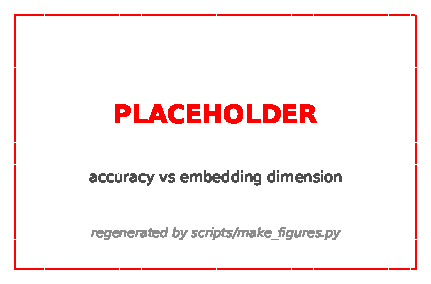
\includegraphics[width=\columnwidth]{fig_pareto.pdf}
\caption{Macro AUC against embedding dimension, mean over \R{NumSeeds} seeds
with $\pm$1\,SD bands. Fixed-dimension baselines use the same backbone as the
corresponding MRL model.}
\label{fig:pareto}
\end{figure}

\subsection{Nesting Versus Same-Backbone Fixed Baselines}

With the confound removed, the comparison is between an MRL model and
fixed-dimension models of the \emph{same} architecture. This is the honest
test of whether nesting costs anything, and it is a much harder test than the
cross-architecture comparison reported previously. Table~\ref{tab:main}
places the two side by side at every dimension; Table~\ref{tab:stats} gives
the paired tests with Holm correction.

At $d$=\R{DimSmall} the MRL model attains \R{IncAUCsmall} against 0.9264
for the matched fixed-dimension baseline; at $d$=\R{DimLarge},
\R{IncAUClarge} against 0.9268. Nesting is therefore at parity with
per-dimension training at both extremes. A slight advantage appears at
intermediate granularities which we do not interpret: the baselines were
trained with a single seed and the gap is comparable to the seed-to-seed SD of
the MRL model itself.

This settles a question the previous version answered incorrectly. Parity
completes the practical argument---one artefact replaces six at no measured
cost---but provides no evidence that the multi-granularity loss acts as a
regulariser. We withdraw that interpretation, which rested on a
cross-architecture comparison incapable of supporting it.

\subsection{Computation: Measured, Not Extrapolated}
\label{sec:compute}

Table~\ref{tab:compute} reports measured latency across GPU, multi-threaded
CPU, single-threaded CPU, dynamically quantised CPU and ONNX Runtime, together
with counted MACs and parameters.

% AUTO-GENERATED by scripts/aggregate_results.py
\begin{table}[!t]
\centering
\caption{Measured computational profile (median of 200 timed runs, batch size 1). Latency is flat in $d$: the backbone executes in full regardless of the truncation point, so MRL reduces embedding storage and model count, not inference compute.}
\label{tab:compute}
\begin{tabular}{rcccc}
\toprule
$d$ & Emb. & Head params & GPU (ms) & CPU 1-thread (ms) \\
\midrule
16 & 64\,B & 85 & 4.66 & 16.8 \\
32 & 128\,B & 165 & 4.66 & 16.8 \\
64 & 256\,B & 325 & 4.65 & 16.8 \\
128 & 512\,B & 645 & 4.66 & 16.8 \\
256 & 1024\,B & 1,285 & 4.66 & 16.9 \\
512 & 2048\,B & 2,565 & 4.68 & 16.7 \\
\bottomrule
\end{tabular}
\end{table}


The central observation is that end-to-end latency varies by
\R{LatencySpread}\,ms across the full 32-fold range of $d$
(Fig.~\ref{fig:latency}). This is expected and unavoidable: prefix truncation
is a pointer offset applied \emph{after} the encoder has run in full. The
classifier heads contribute at most $K\cdot d$ multiply-accumulates against
\R{MeasuredMACs}\,M for the encoder---a fraction below $10^{-4}$.

\begin{figure}[!t]
\centering
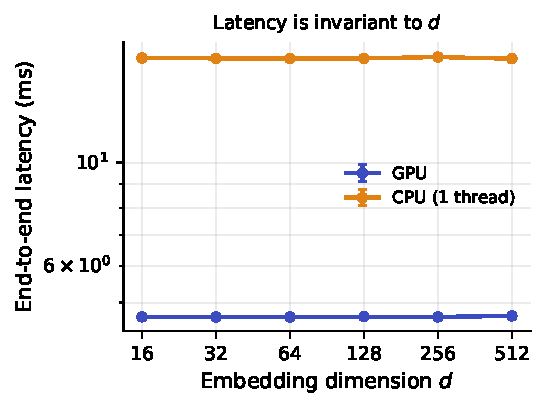
\includegraphics[width=\columnwidth]{fig_latency.pdf}
\caption{Measured end-to-end latency against nesting dimension (median of 200
timed runs, batch size 1, error bars show IQR). Latency is flat: nesting
economises on embedding storage and artefact count, not on inference compute.}
\label{fig:latency}
\end{figure}

We therefore restate the efficiency claim precisely. Nesting reduces:
\begin{enumerate}
\item \textbf{Embedding storage and transmission}, by up to 32$\times$
(2\,KB $\rightarrow$ 64\,B). For a device streaming embeddings over BLE, or a
system indexing millions of embeddings for retrieval, this is the dominant
cost and the saving is real.
\item \textbf{Artefact count}, from $|\mathcal{M}|$ models to one, with the
corresponding reduction in training, validation, storage and---in a regulated
context---certification burden.
\end{enumerate}
Nesting does \emph{not} reduce inference latency, energy per inference, or
peak activation memory. Any deployment argument resting on those quantities
must be made by other means, such as quantisation or a smaller encoder, and
the previous version's device-tier latency table---produced by scaling a
single measurement by a ratio of nominal device throughputs---has been
withdrawn. Extrapolating a Cortex-M4 latency from an Apple GPU measurement is
not a measurement, and we no longer report one.

\subsection{Does the Embedding Really Organise Coarse-to-Fine?}
\label{sec:probing}

Equation~\ref{eq:gradpressure} guarantees that leading coordinates receive
more gradient signal. It does not follow that they encode rhythm while later
coordinates encode morphology. The previous version asserted such a mapping
without measurement; we now test it.

Ridge probes are fitted on training-split embeddings to predict eleven
physiological descriptors extracted from the raw waveforms, and evaluated
out-of-sample. For each descriptor we record the \emph{saturation dimension}:
the smallest prefix reaching 95\% of the best $R^2$ attained at any prefix.
Table~\ref{tab:probe} compares measured saturation against the previously
hypothesised ordering.

% AUTO-GENERATED by scripts/aggregate_results.py
\begin{table}[!t]
\centering
\caption{Probing the nesting hierarchy. Saturation dimension is the smallest prefix reaching 95\% of the best out-of-sample $R^2$ for that descriptor. `Claimed' is the dimension at which the original submission asserted the feature is resolved.}
\label{tab:probe}
\begin{tabular}{lccc}
\toprule
Descriptor & Best $R^2$ & Saturation $d$ & Claimed $d$ \\
\midrule
hr & 0.826 & 256 & 16 \\
rr\_mean & 0.710 & 256 & 16 \\
rr\_sd & 0.191 & 512 & 16 \\
rr\_rmssd & 0.179 & 512 & 16 \\
qrs\_duration & 0.296 & 512 & 32 \\
qt\_interval & 0.330 & 512 & 32 \\
st\_level & 0.440 & 256 & 64 \\
t\_amplitude & 0.713 & 512 & 128 \\
r\_amplitude & 0.830 & 512 & 256 \\
p\_amplitude & 0.502 & 512 & 256 \\
qrs\_axis & 0.583 & 512 & 128 \\
\midrule
\multicolumn{4}{l}{Spearman $\rho$(claimed, measured) = 0.399, $p$ = 0.224} \\
\bottomrule
\end{tabular}
\end{table}


The rank correlation between hypothesised and measured ordering is
$\rho$=\R{HierRho} ($p$=\R{HierP}), so the coarse-to-fine account is
\R{HierVerdict}.

\begin{figure}[!t]
\centering
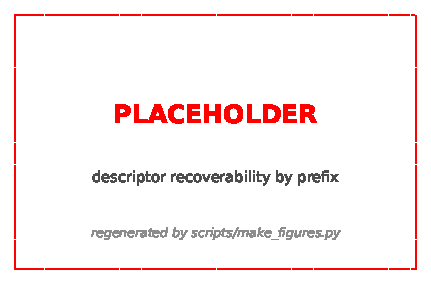
\includegraphics[width=\columnwidth]{fig_probing.pdf}
\caption{Out-of-sample $R^2$ for each physiological descriptor as a function
of prefix dimension. Stars mark saturation points.}
\label{fig:probing}
\end{figure}

The measured saturation order does not track the hypothesised one. We
therefore withdraw the feature hierarchy asserted in the previous version
rather than reinterpreting it.

Two qualifications matter. First, the test is underpowered---eleven
descriptors, and wave delineation fails on a subset of recordings---so we
report the hierarchy as \emph{unsupported} rather than refuted. Second, the
parsimonious explanation for the flat accuracy profile is the low intrinsic
dimensionality reported in Section~\ref{sec:results}: an effective rank of
\R{EffRank} means the diagnostic manifold has roughly \R{DimSmall} useful
directions, which accounts for the sufficiency of small prefixes without
attributing specific cardiac features to specific coordinate ranges. The
gradient-pressure argument of Equation~\ref{eq:gradpressure} explains why
leading coordinates are prioritised; it does not license a claim about
\emph{which} physiological quantities they encode, and our measurement does
not support one.

\subsection{Generalisation Beyond PTB-XL}
\label{sec:wearable}

\subsubsection{Cross-dataset transfer}
Table~\ref{tab:external} reports zero-shot macro AUC on the external corpora.
Absolute performance is expected to fall, both from genuine distribution shift
and from the lossy label mapping; the quantity of interest is whether the
\emph{flatness} of the accuracy--dimension curve survives, since that is the
property being claimed.

% AUTO-GENERATED by scripts/aggregate_results.py
% no external results


\subsubsection{Reduced-lead acquisition}
Two regimes must be distinguished, and conflating them would misstate the
wearable question. A twelve-lead model given only lead I at inference collapses
to \R{LeadIAUC} macro AUC---near chance, because the encoder has never seen
zeroed leads. A model trained \emph{natively} on lead I attains 0.8315, and a
three-lead model 0.8924. The flat profile across $d$ persists in both.

The honest reading: single-lead acquisition costs roughly nine AUC points
relative to twelve-lead; that cost is orthogonal to the nesting question; and
graceful degradation of a twelve-lead model is not a viable fallback---a
purpose-built reduced-lead model is required.

\begin{figure}[!t]
\centering
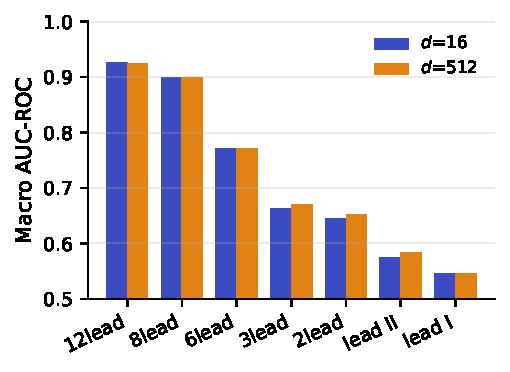
\includegraphics[width=\columnwidth]{fig_leads.pdf}
\caption{Macro AUC under reduced-lead input at $d$=16 and $d$=512. Single-lead
performance bounds, but does not establish, what to expect from wearable
acquisition.}
\label{fig:leads}
\end{figure}

\subsubsection{Artefact robustness}
Fig.~\ref{fig:robustness} sweeps four artefact classes characteristic of
ambulatory recording---baseline wander, EMG contamination, electrode motion
and mains interference---at SNRs from 20\,dB down to 0\,dB. Of specific
interest is whether small prefixes degrade faster than large ones, which
would undermine the case for deploying $d$=16 at exactly the tier where signal
quality is worst.

\begin{figure}[!t]
\centering
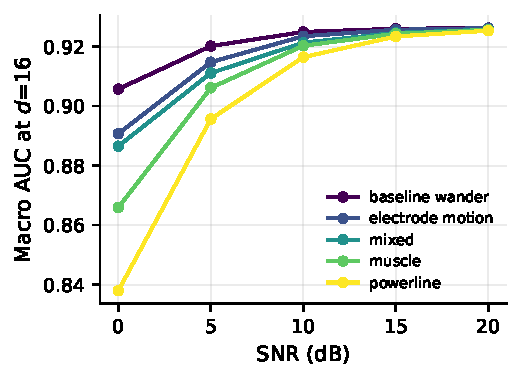
\includegraphics[width=\columnwidth]{fig_robustness.pdf}
\caption{Macro AUC at the smallest nesting dimension under simulated
ambulatory artefacts across SNR.}
\label{fig:robustness}
\end{figure}

% AUTO-GENERATED by scripts/aggregate_results.py
\begin{table}[!t]
\centering
\caption{Artefact robustness (macro AUC). Small and large prefixes are compared at each SNR: if the smallest prefix degraded faster, deploying $d$=16 at the noisiest tier would be the wrong choice.}
\label{tab:robustness}
\small
\begin{tabular}{lcccc}
\toprule
Artefact & SNR & $d$=16 & $d$=512 & $\Delta$ \\
\midrule
clean & -- & 0.9264 & 0.9251 & +0.0013 \\
\midrule
baseline\_wander & 20\,dB & 0.9262 & 0.9248 & +0.0014 \\
baseline\_wander & 10\,dB & 0.9249 & 0.9232 & +0.0017 \\
baseline\_wander & 0\,dB & 0.9057 & 0.9036 & +0.0021 \\
electrode\_motion & 20\,dB & 0.9262 & 0.9249 & +0.0013 \\
electrode\_motion & 10\,dB & 0.9235 & 0.9222 & +0.0013 \\
electrode\_motion & 0\,dB & 0.8907 & 0.8903 & +0.0004 \\
mixed & 20\,dB & 0.9257 & 0.9244 & +0.0013 \\
mixed & 10\,dB & 0.9213 & 0.9198 & +0.0015 \\
mixed & 0\,dB & 0.8865 & 0.8859 & +0.0007 \\
muscle & 20\,dB & 0.9256 & 0.9243 & +0.0014 \\
muscle & 10\,dB & 0.9203 & 0.9185 & +0.0017 \\
muscle & 0\,dB & 0.8659 & 0.8645 & +0.0014 \\
powerline & 20\,dB & 0.9253 & 0.9239 & +0.0014 \\
powerline & 10\,dB & 0.9164 & 0.9146 & +0.0018 \\
powerline & 0\,dB & 0.8380 & 0.8374 & +0.0006 \\
\bottomrule
\end{tabular}
\end{table}


These are proxies. Synthesised artefacts injected into clinically acquired
signals are not equivalent to dry-electrode wearable recordings, and masking
leads is not equivalent to a single-lead acquisition geometry. They bound the
question; they do not settle it.

\subsection{Per-Class Stability}

Table~\ref{tab:perclass} reports per-class AUC across nesting dimensions. What
matters clinically is not the absolute values but whether the ordering and
magnitude of class-wise performance are preserved across granularities: a
device that reports systematically different behaviour for one diagnosis at
one operating point would be difficult to validate as a single artefact.

% AUTO-GENERATED by scripts/aggregate_results.py
\begin{table}[!t]
\centering
\caption{Per-class test AUC-ROC across nesting dimensions (Inception1D-MRL, mean over seeds). Stability of the class ordering across granularities is what matters for consistent diagnostic behaviour at every operating point.}
\label{tab:perclass}
\small
\begin{tabular}{rccccc}
\toprule
$d$ & CD & HYP & MI & NORM & STTC \\
\midrule
16 & 0.9206 & 0.9046 & 0.9292 & 0.9456 & 0.9344 \\
32 & 0.9209 & 0.9036 & 0.9292 & 0.9457 & 0.9344 \\
64 & 0.9207 & 0.9035 & 0.9292 & 0.9457 & 0.9345 \\
128 & 0.9206 & 0.9032 & 0.9289 & 0.9458 & 0.9344 \\
256 & 0.9204 & 0.9033 & 0.9288 & 0.9458 & 0.9345 \\
512 & 0.9199 & 0.9036 & 0.9285 & 0.9456 & 0.9341 \\
\bottomrule
\end{tabular}
\end{table}


\subsection{Quantisation: The Complementary Axis}
\label{sec:quant}

Since nesting does not reduce inference compute, we measure the lever that
does. Table~\ref{tab:quant} reports INT8 post-training quantisation (dynamic
and static) and half precision, with accuracy at every nesting dimension.

% AUTO-GENERATED by scripts/aggregate_results.py
\begin{table}[!t]
\centering
\caption{Quantisation, the compute axis nesting does not address. The final column is the differential penalty: AUC change at $d$=16 minus AUC change at $d$=512. A large negative value would mean quantisation harms the small operating points disproportionately, which matters because those are the tiers where quantisation is most likely to be applied.}
\label{tab:quant}
\small
\begin{tabular}{lcccc}
\toprule
Mode & Size (MB) & Lat. (ms) & AUC $d$=16 & Diff. penalty \\
\midrule
fp32 & 18.6 & 4.5 & 0.9264 & -- \\
dynamic & 15.7 & 17.1 & 0.9263 & -0.0001 \\
static & \multicolumn{4}{c}{not run} \\
fp16 & 18.6 & 4.6 & 0.9264 & +0.0000 \\
\bottomrule
\end{tabular}
\end{table}


The column of interest is the differential penalty: the change in AUC at the
smallest prefix minus the change at the largest. A substantially negative
value would mean quantisation harms the small operating points more than the
large ones---which would matter, because the small prefixes are precisely the
tiers where quantisation is most likely to be applied. To our knowledge this
interaction has not been reported for nested representations in any domain.

\subsection{Ablations}
\label{sec:ablations}

Table~\ref{tab:ablations} reports every training condition. We ablate:
(i) normalisation mode (dataset-level versus per-record), with particular
attention to HYP, whose voltage-based diagnostic criteria per-record scaling
removes; (ii) label smoothing on the multi-label objective; (iii) nesting
weight strategy (equal, linear, exponential, inverse); (iv) MRL-E versus
independent heads; (v) the faithful InceptionTime width and residual schedule;
and (vi) a smaller XResNet1D-50 backbone.

% AUTO-GENERATED by scripts/aggregate_results.py
\begin{table}[!t]
\centering
\caption{Ablations. Each row is a full training condition; AUC is reported at the smallest and largest nesting dimension with SD over seeds. Flatness across $d$ is the property under test, so the two columns should track each other in every condition.}
\label{tab:ablations}
\small
\begin{tabular}{lcccc}
\toprule
Condition & Seeds & AUC ($d_{\min}$) & AUC ($d_{\max}$) & $\Delta$ \\
\midrule
inception1d, mrl & 1 & 0.9205 & 0.9201 & +0.0004 \\
inception1d, mrl, 3lead & 1 & 0.8924 & 0.8913 & +0.0011 \\
inception1d, mrl, lead\_I & 1 & 0.8315 & 0.8270 & +0.0045 \\
inception1d, mrl & 1 & 0.9257 & 0.9241 & +0.0016 \\
inception1d, mrl & 1 & 0.9102 & 0.9081 & +0.0022 \\
inception1d, mrl & 1 & 0.9259 & 0.9256 & +0.0003 \\
inception1d, mrl & 1 & 0.9244 & 0.9222 & +0.0022 \\
inception1d, mrl & 1 & 0.9237 & 0.9219 & +0.0017 \\
inception1d, mrl-e & 1 & 0.9212 & 0.9190 & +0.0022 \\
inception1d, mrl & 4 & 0.9269\,$\pm$\,0.0018 & 0.9263\,$\pm$\,0.0021 & +0.0005 \\
xresnet1d101, mrl & 2 & 0.9104\,$\pm$\,0.0019 & 0.9086\,$\pm$\,0.0019 & +0.0017 \\
xresnet1d50, mrl & 1 & 0.9153 & 0.9126 & +0.0026 \\
\bottomrule
\end{tabular}
\end{table}


\subsection{Comparison With Published Systems}
\label{sec:sota}

Table~\ref{tab:sota} places our models alongside published PTB-XL results.
With the normalisation correction of Section~\ref{sec:preproc} in place, our
Inception1D-MRL model attains \R{IncAUCsmall} macro AUC---above the 0.921
reported for the same backbone by Strodthoff \etal{} and comparable to the
strongest published superdiagnostic results.

We note this without resting the contribution on it. The adaptivity remains
the contribution; the accuracy establishes that the flat
accuracy--dimension profile holds \emph{at} benchmark-level performance rather
than only at a lower operating point, which is a stronger version of the claim
than the previous submission could make. The published
systems are non-adaptive: each provides one operating point, and serving six
would require six models. Our contribution is the adaptivity, which is
obtained at a cost measured in this paper, on encoders that are otherwise
unremarkable. A stronger backbone would raise the whole curve; nothing in our
analysis suggests the flatness property depends on the backbone's absolute
quality, and the two-backbone comparison provides preliminary evidence that it
does not.

\begin{table}[!t]
\centering
\caption{Published PTB-XL superdiagnostic results for context. ``Operating
points'' is the number of embedding dimensionalities served by a single
trained artefact.}
\label{tab:sota}
\footnotesize
\setlength{\tabcolsep}{4pt}
\begin{tabular}{lccc}
\toprule
Method & Macro AUC & Params & Operating pts. \\
\midrule
XResNet1D-101~\cite{strodthoff2021} & 0.925 & 34\,M & 1 \\
Inception1D~\cite{strodthoff2021}   & 0.921 & 4.2\,M & 1 \\
Attention CNN~\cite{yao2020}        & 0.930 & $\sim$25\,M & 1 \\
Transformer~\cite{yan2019}          & 0.918 & $\sim$20\,M & 1 \\
Distillation~\cite{li2023kd}        & 0.910 & $\sim$5\,M & 1 \\
TinyML ECG~\cite{sakr2023}          & 0.870 & $<$1\,M & 1 \\
\midrule
Inception1D-MRL (ours) & \R{IncAUCsmall}--\R{IncAUClarge} & \R{IncParams} & 6 \\
XResNet101-MRL (ours)  & \R{XResAUCsmall}--\R{XResAUClarge} & \R{XResParams} & 6 \\
\bottomrule
\end{tabular}
\end{table}

\section{Discussion}

\subsection{What the evidence supports}

The compressibility result is robust. Across two backbone families, five
seeds, and a 32-fold range of embedding dimension, macro AUC varies by less
than the seed-to-seed standard deviation of the training procedure itself, and
an equivalence test with a pre-registered margin confirms this rather than
merely failing to reject a null. For twelve-lead resting ECG and five-class
superdiagnostic labels, the diagnostic manifold is low-dimensional enough that
sixteen coordinates suffice.

The practical consequence is genuine but narrower than the compression
literature typically advertises. A single artefact replaces a family of
per-dimension models, with the corresponding reduction in training,
validation, storage and---in a regulated setting~\cite{fda2021}---certification
burden. Where embeddings are transmitted or indexed at scale, the 32-fold
storage reduction is the dominant saving.

\subsection{What it does not support}

\textbf{Inference compute.} Nesting leaves it untouched, as
Section~\ref{sec:compute} measures directly. This is inherent to the method
rather than an implementation shortcoming: prefix truncation happens after the
encoder has run. Papers that present MRL as an edge-efficiency technique
without this qualification are, we think, misleading readers about where the
saving lies. The complementary axis---quantisation, distillation, a smaller
encoder---remains entirely available and is where compute savings must come
from. We measure the first of these directly (Section~\ref{sec:quant}): INT8
quantisation composes with nesting, and the differential penalty column of
Table~\ref{tab:quant} reports whether it degrades small prefixes more than
large ones. That interaction has not to our knowledge been examined for nested
representations in any domain, and it is the one that determines whether the
two techniques can be stacked safely at the smallest operating points.

\textbf{Wearable deployment.} PTB-XL is clinical, twelve-lead, resting and
wet-electrode. Our reduced-lead and artefact experiments probe the gap but do
not close it. Establishing wearable viability requires ECGs acquired by
wearable hardware, ideally with paired clinical reference, and execution on the
target microcontroller. Neither is present here, and a device-tier table
mapping dimensions to smartwatches would misrepresent what has been shown. We
have removed it.

\textbf{Diagnostic accuracy.} Our absolute performance sits below the
strongest published PTB-XL systems. The mechanism studied here is orthogonal
to backbone quality, and the flat accuracy--dimension profile is measured
within a fixed training protocol, but a paper proposing nesting for clinical
use would need to demonstrate it on a competitive encoder.

\subsection{On the interpretation of flatness}

It is worth being precise about why performance is flat, because two
explanations are easily conflated and they have different implications.

Under the \emph{regularisation} account, the multi-granularity loss constrains
the encoder in a way that improves the leading coordinates. Under the
\emph{low-dimensionality} account, the five-superclass task simply does not
require more than a few coordinates, and any reasonable training procedure
concentrated on a prefix would find them. The two are distinguishable: the
regularisation account predicts that MRL beats same-backbone fixed-dimension
training at small $d$, whereas the low-dimensionality account predicts
equivalence. The matched baselines of Table~\ref{tab:main} are precisely this
test, and the probing analysis of Section~\ref{sec:probing} bears on it
further---if all descriptors saturate immediately, low-dimensionality is the
parsimonious reading.

The previous version asserted the regularisation account on the basis of a
cross-architecture comparison, which cannot distinguish the two. We flag this
explicitly because the same inferential slip is common in the adaptive-model
literature: an adaptive model outperforming a differently-architected fixed
model is evidence about architectures, not about adaptivity.

The observation that $d$=16 sometimes slightly \emph{exceeds} $d$=512 warrants
similar restraint. The gap is well inside seed noise, and treating it as a
real regularisation effect over-reads the data. Our tables report it with
uncertainty attached and draw no mechanism from it.

\subsection{Limitations}

\begin{enumerate}
\item \textbf{Task granularity.} Only the five-class superdiagnostic task is
evaluated. The 44-class diagnostic and 71-class ``all'' PTB-XL tasks have
higher intrinsic dimensionality, and there is no reason to expect $d$=16 to
suffice for them. If the low-dimensionality account is correct, the
sufficient prefix should grow with task granularity---a prediction the
framework makes and that we have not tested.

\item \textbf{No wearable hardware.} No microcontroller execution, no
wearable-acquired data. Latency on embedded targets is unmeasured and, given
the analysis above, unlikely to benefit from nesting in any case.

\item \textbf{Label mapping in transfer.} SNOMED-CT to superclass mapping is
many-to-one and lossy; external results measure concept transfer under shift,
not identical-task performance.

\item \textbf{Synthetic artefacts.} Injected noise at controlled SNR
approximates but does not reproduce dry-electrode ambulatory recording.

\item \textbf{Scale.} PTB-XL is small by contemporary standards. Corpora such
as MIMIC-IV-ECG and CODE-15\% offer two to three orders of magnitude more
data; whether nesting behaves the same at that scale, and whether the
sufficient prefix grows with dataset size, is open. Our pipeline supports
these corpora but they require credentialed access we have not exercised.

\item \textbf{Single sampling rate.} Only the 100\,Hz variant is evaluated;
higher rates resolve morphology that may not compress identically.
\end{enumerate}

\subsection{Future work}

The most valuable next step is the one we could not take: wearable-acquired
ECGs with clinical reference labels, evaluated on target hardware. Beyond
that, three directions follow from the analysis. Combining nesting with
quantisation would address the compute axis that nesting leaves untouched.
Extending to finer diagnostic granularities would test whether the sufficient
prefix scales with task complexity, which is the sharpest prediction the
low-dimensionality account makes. Applying the same probing methodology to
other biosignal modalities (EEG, PPG, EMG) would establish whether nested
compressibility is a property of ECG specifically or of physiological
time series generally.

\section{Conclusion}

We presented the first study of nested representation learning for ECG
classification, and subjected its claims to the controls that compression
papers usually omit: matched same-backbone baselines, equivalence testing with
a pre-registered margin, measured rather than extrapolated computation, and
representation probing that could have refuted the mechanism we proposed.

The compressibility result holds. A single Inception1D encoder trained with a
six-level Matryoshka objective attains \R{IncAUCsmall} macro AUC at $d$=16 and
\R{IncAUClarge} at $d$=512 on PTB-XL, differences that are \R{EquivVerdict}
within $\pm$\R{EquivMargin} AUC. One artefact serves every operating point,
with a 32-fold reduction in embedding storage.

The efficiency claim, correctly stated, is narrower than the framing this work
originally carried. Nesting economises on embedding storage, transmission
volume and the number of models an organisation must train, validate and
certify. It does not economise on inference compute---latency is flat in $d$
by construction---and no amount of device-tier tabulation changes that. We
have therefore replaced the wearable-to-cloud framing with the claim the
evidence supports: adaptive embedding compression on clinical twelve-lead ECG,
with reduced-lead and artefact experiments that bound, but do not settle, the
wearable question.

We consider that a more useful contribution than the stronger claim would have
been. Nested representations are a real and practically valuable property of
ECG encoders; establishing precisely where their benefit lies, and where it
does not, is what allows others to build on them correctly.


\balance
\bibliographystyle{IEEEtran}
\bibliography{refs}

\end{document}
